% !TeX root = main.tex
\lecture{2}{Thu 22 Jan 2026 13:00}{Matter II: Atomic Physics and LJP}

\section{Atomic Sizes}
As we increase proton number, we might expect that the atomic radius increases (as there's physically more stuff). We might expect that adding more electrons would expect a corresponding increase in the atomic radius to fit these extra electrons.

This doesn't actually prove to be true, and atomic size and properties are generally determined by the outermost electrons, and atomic radius stays mostly constant.

\begin{figure}[H]
    \centering
    
\includegraphics[width=0.75\textwidth]{figures/lec02-01.png}
     \caption{Variation of Atomic Radius with Atomic Number}
\end{figure}

We do see a large increase in atomic radius for the group one metals, where the outermost electron is very weakly attracted to the nucleus (is easily ionised). For an exam, we can consider atomic radius to be approximately $10^{-10}$.

We see a similar trend when considering ionisation energy (the energy required to remove the outermost electron):

\begin{figure}[H]
    \centering
    
\includegraphics[width=0.75\textwidth]{figures/lec02-02.png}
     \caption{}
\end{figure}

This is approximately the same for the all atomic numbers, with the exception of noble gases (which are extremely difficult to ionise as a result of having full capacity outer shells).

This doesn't apply however to the nuclear radius, $R$, as the nucleus is compressed to a much higher degree, so there's not space to fit additional nucleons without increasing radius. For atomic radius $A$, and modelling the nucleus as a sphere, we get:
\[
    R = r_0 A^{\frac{1}{3}}
\]

Where $r_0 = 1.2 \times 10^{-15}m = 1.2 \si{\femto\metre}$ is a constant.

\section{Atomic Masses}
Given the extremely small mass scales, we generally give masses of atoms or molecules in terms of atomic mass units, amu, where:
\[
    1 \text{amu} = 1.66 \times 10^{-27} \si{\kilo\gram}
\]

This is defined as $1/12$th the mass of a Carbon-12, ${}^{12} C$ atom. The atomic mass of Carbon-12 is thus $12$amu, however a proton and neutron each have mass $1.007$amu and $1.009$amu respectively. Why is there a discrepancy if we add the masses of the individual nucleons?

This is because, when combining these nucleons into a nucleus, some of this mass is converted into energy. This is called ``binding energy'' and is used to hold the nucleus together.

\subsection{Moles}
A mole ($\si{\mole}$) is an SI base unit used to described the amount of a substance. 1 mole of a substance is defined by Avagadro's number, $N_A = 6.022 \times 10^{23}$, where one mole has $N_A$ atoms/molecules. We again use Carbon 12, as 12 grams of Carbon-12 has $N_A$ atoms.

We further have:
\[
    \text{amount, mol} = \frac{N}{N_A}
\]
\[
    \text{amount, mol} = \frac{\text{Mass}}{\text{Atomic Mass}}
\]

For gasses, one mole occupies exactly $22.4$L or $22.4\si{dm^3}$ at standard temperature and pressure ($0\si{\degreeCelsius}$, $10^5\si{Pa} = 1\si{atm}$), regardless of the gas in consideration.

\section{Rayleigh's Oil Drop Measurement}
Rayleigh conducted an experiment where he took a large volume of water, and placed a drop of olive oil (of known volume $V$) on top. He postulated that, due to the nature of olive oil being long-chained hydrocarbons, the oil would spread out perfectly thinly, and produce a layer exactly one atom tall.

He said that this would form a circular layer of radius $R$ and height $d$. If we take the film to be a cylinder (and $d$ is too small to measure directly), we can measure $R$ and use the known volume to determine $d$:
\[
    V = \pi R^2 d \implies d = \frac{V}{\pi R^2}
\]

When he carried this out, he determined the atomic radius \footnote{Strictly, an upper limit for the radius}, as $\sim 1 \si{nm}$, i.e. being one order of magnitude out. This wasn't bad for how rudimentary the experiment was!

\section{Latent Heat}
We know that there has to be some kind of force between two atoms. If we consider a diatomic molecule, separating these atoms from each other to infinity requires some amount of energy $\epsilon$. Because there are two atoms, the work done per atom is $\epsilon / 2$.

Lets consider a more complex example with many more atoms (i.e. converting a solid to liquid):
\begin{figure}[H]
    \centering
    
\includegraphics[width=0.75\textwidth]{figures/lec02-03.png}
     \caption{}
\end{figure}

In this case, extracting the red atom from all its $12$ nearest neighbours will take $12 \epsilon / 2$. We should additionally consider the $6$ next nearest neighbours and so and so on. Each increase in number of $n$th next nearest neighbours has a decreasing impact in the force required, so leads to diminishing returns. In this course, we often ignore he next nearest neighbours and further. If asked to estimate, we use $6-10$ for a liquid, and $8-12$ for a solid.

While we're considering this in a solid, lets use it as an approximation for a liquid. The latent heat of vaporisation $L (\si{J kg})$ is the amount of heat required to completely vaporise a liquid into a gas.

\[
    L = 12 \epsilon / 2 \times \frac{\text{number of atoms}}{\text{mass of material, kg}}
\]

And the number/mass is given by:
\[
   \frac{\text{kg}}{\text{atoms}} = \rho \times d^3 \implies \frac{\text{atoms}}{\text{kg}} = \frac{1}{\rho d^3} 
\]

Hence:
\[
    d = \sqrt[3]{\frac{1}{\text{atoms per kg} \times \rho}}
\]

\section{Forces Between Atoms}
What causes the forces between atoms? It can't be the electrostatic (coulomb) force, as atoms are electrically neutral.

It can't be the nuclear force, as the range is too small. Likewise, it can't be the weak force as this mediates the wrong particles and has an even smaller range.

Finally, it can't be gravitational as atoms have far too low a mass for the gravitational force to have any real impact.

Even though the electrostatic component has no impact, the electromagnetic force as a whole can.

\subsection{Water Example}
Oxygen is slightly electronegative, while hydrogen is not. This means that if we have a $H_2 O$ water molecule, the electrons will be pulled ever so slightly closer to the oxygen and away from the hydrogen. Across the whole atom, this causes a slight charge on each side of the atom:

\begin{figure}[H]
    \centering
    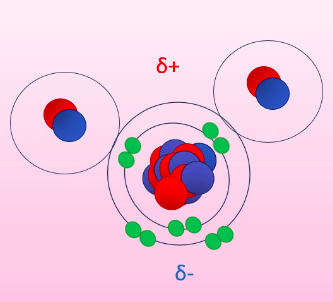
\includegraphics[width=0.75\textwidth]{figures/lec02-04.png}
     \caption{}
\end{figure}

Water is ``polar molecule'' and forms a permanent dipole, where the positive and negative poles of molecules attract.

\section{``Normal'' Atoms}
This only works for some atoms. A block of iron for example cannot be explained by this, as all the atoms are the same, so have equivalent electronegativity.

Here, fluctuations in the electron cloud cause an instantaneous dipole to form. This may be very brief, but lasts for sufficiently long to impact another atom. This atom has electron distribution impacted by this force, causing it to be become a dipole. This creates a field which impacts the original atom etc. This causes the atoms to be stuck as instantaneous dipoles, resulting in a net attractive force called the Van der Waal's force.

As the electric field due to a dipole goes as $|E| \propto 1/r^3$, the induced dipole in the firs atom depends on the strength of its dipole field and the size of the induced dipole in the second atom:

\[
    |E| = \frac{1}{r^3} \frac{1}{r^3} = \frac{1}{r^6}
\]

The force induced by these dipoles explains attraction for non-polar molecules. Force between two atoms is considered positive (by convention) if they repel and negative if they attract.

However, the fact that atoms have a consistent interatomic spacing and do not collapse into black holes suggests that there is some kind of repulsive force that keeps them at fixed distances.

We can infer that this force must be very strong at small distances, but much weaker at larger distances.

\section{LJ Potential}

We can divide particles into fermions (half integer spin) and bosons (integer spin). The wave fuction of a boson is symmetric about $y$, so overlapping two bosons causes superposition. Fermions are antisymmetric (i.e. a sine wave). This means that two fermions in the same position causes destructive interference, with a net wave function of $0$. 

This means that two fermions in the same quantum state (same wave function) cannot share a position, and have a force repelling each other should they try. We approximate this as a potential of the form:
\[
    V \propto \frac{1}{r^{12}}
\]

Lennard-Jones combined these, describing the net potential of the form:

\[
    V_{LJ} = \frac{A}{r^{12}} - \frac{B}{r^{6}}
\]




